\documentclass[11pt]{standalone}
\usepackage{amssymb}
\usepackage{amsmath}
\usepackage[no-math]{fontspec}
\usepackage{unicode-math}
\usepackage{libertinus}
\usepackage{pgf,xcolor}
\usepackage{tikz}
\usetikzlibrary{arrows.meta, backgrounds}
\usepackage{pgfplots}
\pgfplotsset{compat=newest}

\setmainfont{Libertinus Serif}
\setmathfont{Libertinus Math}

\definecolor{my_darkgray}{HTML}{484949}
\definecolor{my_lightgray}{HTML}{F3F4F4}
\definecolor{my_darkblue}{HTML}{005A94}
\definecolor{my_lightblue}{HTML}{CCDEE9}
\definecolor{my_yellow}{HTML}{FFEC7F}
\definecolor{my_red}{HTML}{E60000}
\definecolor{my_orange}{HTML}{E87846}

\begin{document}

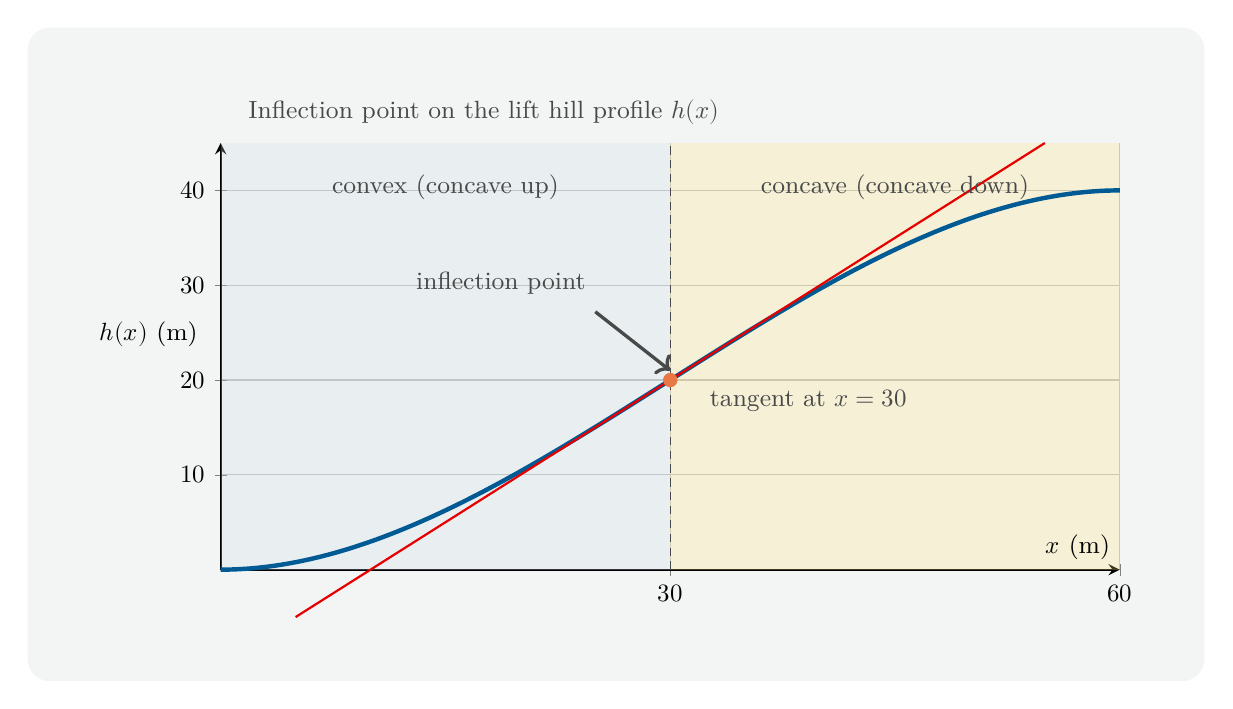
\begin{tikzpicture}[
    show background rectangle,
    background rectangle/.style={fill=my_lightgray, rounded corners=8pt},
    inner frame sep=0.8cm
]

\begin{axis}[
    width=13cm,
    height=7cm,
    axis lines = center,
    xlabel = {$x$ (m)},
    ylabel = {$h(x)$ (m)},
    xmin=0, xmax=60,
    ymin=0, ymax=45,
    xtick={0,30,60},
    ytick={0,10,20,30,40},
    grid = major,
    axis line style={thick},
    ticklabel style={font=\small},
    label style={font=\small},
    ylabel style={
      at={(axis description cs:-0.08,0.5)},
      anchor=south
    },
    clip=false,
]

% background shading: convex region [0, 30]
\fill[my_lightblue, opacity=0.25]
  (axis cs:0,0) rectangle (axis cs:30,45);

% background shading: concave region [30, 60]
\fill[my_yellow, opacity=0.25]
  (axis cs:30,0) rectangle (axis cs:60,45);

% lift hill height profile h(x) = x^2/30 - x^3/2700
\addplot[
    draw=my_darkblue,
    ultra thick,
    samples=400,
    domain=0:60
]
{0.0333333333*x^2 - 0.00037037037*x^3};

% inflection point at x = 30: h(30) = 20
\addplot[
    only marks,
    mark=*,
    mark size=2.4pt,
    draw=my_orange,
    fill=my_orange
]
coordinates {(30,20)};

% vertical dashed line at x = 30
\addplot[
    draw=my_darkgray,
    densely dashed,
    very thin
]
coordinates {(30,0) (30,45)};

% tangent at x = 30: slope 1, equation y = x - 10
\addplot[
    draw=my_red,
    thick,
    domain=5:55,
    samples=2
]
{x - 10};

% region labels (inside plot)
\node[anchor=south, font=\small, my_darkgray]
  at (axis cs:15,38)
  {convex (concave up)};

\node[anchor=south, font=\small, my_darkgray]
  at (axis cs:45,38)
  {concave (concave down)};

% inflection point label with arrow
\node[anchor=south east, font=\small, my_darkgray]
  at (axis cs:25,28)
  {inflection point};

\draw[->, very thick, my_darkgray]
  (axis cs:25,27.2) -- (axis cs:30,21);

% small annotation for tangent
\node[anchor=north west, font=\small, my_darkgray]
  at (axis cs:32,20)
  {tangent at $x = 30$};

\node[anchor=south west, font=\small, my_darkgray]
  at (rel axis cs:0.02,1.02)
  {Inflection point on the lift hill profile $h(x)$};

\end{axis}

\end{tikzpicture}

\end{document}